\documentclass[12pt]{article}
\usepackage[a4paper,margin=1in]{geometry}
\usepackage{setspace}
\usepackage{graphicx}
\usepackage{amsmath}
\usepackage{siunitx}
\usepackage{caption}
\usepackage{url}

\doublespacing
\setlength{\parskip}{0.8em}

\begin{document}


\begin{center}
\textbf{\Large Verifying the Ideal Gas Law in a Pressurized Tank} \\[0.5em]
Kevin Peng (1011043238), Boya Zhang (1010855638), Yang Yang Zhang (1011437786)\\[0.5em]
CHE260 PRA 0101 \\
Ideal Gas Law Lab \\
October 1st, 2025 \\
\end{center}

\section*{Abstract}
Validating the ideal-gas assumption is essential for simplifying thermodynamic modeling in engineering systems.
The ideal gas law assumes a compressibility factor \( Z = 1 \), meaning the gas molecules are sufficiently far apart that intermolecular forces and molecular volumes are negligible. Real gases deviate from this ideal behavior at high pressures or low temperatures, but under typical laboratory conditions, air behaves approximately as an ideal gas.
This experiment applied the Ideal Gas Law to determine the initial mass and volume of air in a pressurized tank and to examine how closely the real world behavior matches the ideal gas model under laboratory conditions. The mass of air transferred was determined by integrating the measured mass-flow-rate data using a Riemann-sum approximation coded in Python. The total transferred mass was \SI{0.030496}{\kilogram}, corresponding to a tank volume of \SI{7.007e-3}{\metre\cubed}. The results confirmed that the air’s compressibility factor was approximately unity (\(Z = 0.997 \pm 0.003\)), validating the ideal-gas assumption. Experimental error was dominated by pressure-gauge calibration and sensor lag, but the overall results were consistent with theoretical expectations.

\section*{Introduction}
The Ideal Gas Law,
\[
PV = m R T,
\]
relates pressure, volume, mass, and temperature for a gas whose molecules are assumed to have negligible volume and no intermolecular forces. This law underpins a wide range of thermodynamic analyses, from chemical process design to energy systems. The objective of this experiment was to (1) calculate the mass and volume of air in a storage tank using measured pressure and temperature data, and (2) verify the ideal-gas assumption by comparing the observed compressibility factor \(Z\) with unity. Understanding how the Ideal Gas Law can be applied to real laboratory data is fundamental to quantifying energy and mass balances in engineering systems.

\section*{Experimental Method}
The apparatus consisted of two rigid tanks connected by a valve system, pressure transducers, thermocouples, and a mass-flow meter.

\begin{figure}[h!]
\centering
\includegraphics[width=0.8\textwidth]{apparatus.png}
\caption{A photograph of the experimental apparatus showing the two tanks, pressure gauges, thermocouples, and valve system.}
\label{fig:apparatus}
\end{figure}

In part 1 of the experiment, the left tank was pressurized to 40 psi gauge pressure while the right tank was evacuated to -6 psi.
Two methods were used to equilibrate the tanks:
(1) rapid expansion using the center solenoid valve, and
(2) slow expansion using a partially-opened micrometer needle valve.
The tanks were allowed to reach both pressure and thermal equilibrium while LabVIEW recorded pressure and temperature data over time.

In part 2 of the experiment, the left tank was pressurized to 40 psi gauge pressure while measuring the mass flow rate of incoming air. 
Data was logged in LabVIEW for time, pressure, temperature, and mass flow rate until pressure and temperature stabilized.

A Python script was used to numerically integrate the mass flow rate \(\dot m(t)\) with respect to time to obtain the total transferred mass:
\[
m = \int_{t_0}^{t_f} \dot m(t)\,dt.
\]
This integral was approximated using a left-hand Riemann sum:
\[
m \approx \sum_{i=1}^{N-1} \dot m_i \,(t_{i+1}-t_i).
\]
All measured pressures were converted from gauge to absolute units by adding atmospheric pressure measured with the laboratory manometer. Temperatures were converted to Kelvin for calculations. Air was assumed ideal with a gas constant of \(R = 0.2870~\si{kJ/(kg\cdot K)}\).

\section*{Results and Discussion}


\subsection*{Volume Ratio of the Tanks}
The volume ratio between the two tanks can be determined from the ideal gas law and the conservation of mass. Let the initial state of the left tank be $(P_1, V_1, T)$ and the right tank be at vacuum (or negligible pressure), so its initial state is not relevant to the total moles of gas. The final state is an equilibrium state with pressure $P_f$ across both tanks, so the total volume is $V_1 + V_2$, and the temperature is the same, $T$.

Since the temperature is constant before and after mixing, the number of moles is conserved. The ideal gas law for the initial state (gas only in the left tank) is:
\[ P_1 V_1 = n R T \]
For the final state (gas in both tanks):
\[ P_f (V_1 + V_2) = n R T \]
Equating the expressions for $nRT$:
\[ P_1 V_1 = P_f (V_1 + V_2) \]
Let $V_1$ be the left-tank volume and $V_2$ be the right-tank volume. Solving for the volume ratio $V_2/V_1$:
\[ \frac{V_2}{V_1} = \frac{P_1}{P_f} - 1 \]

\begin{figure}[h!]
\centering
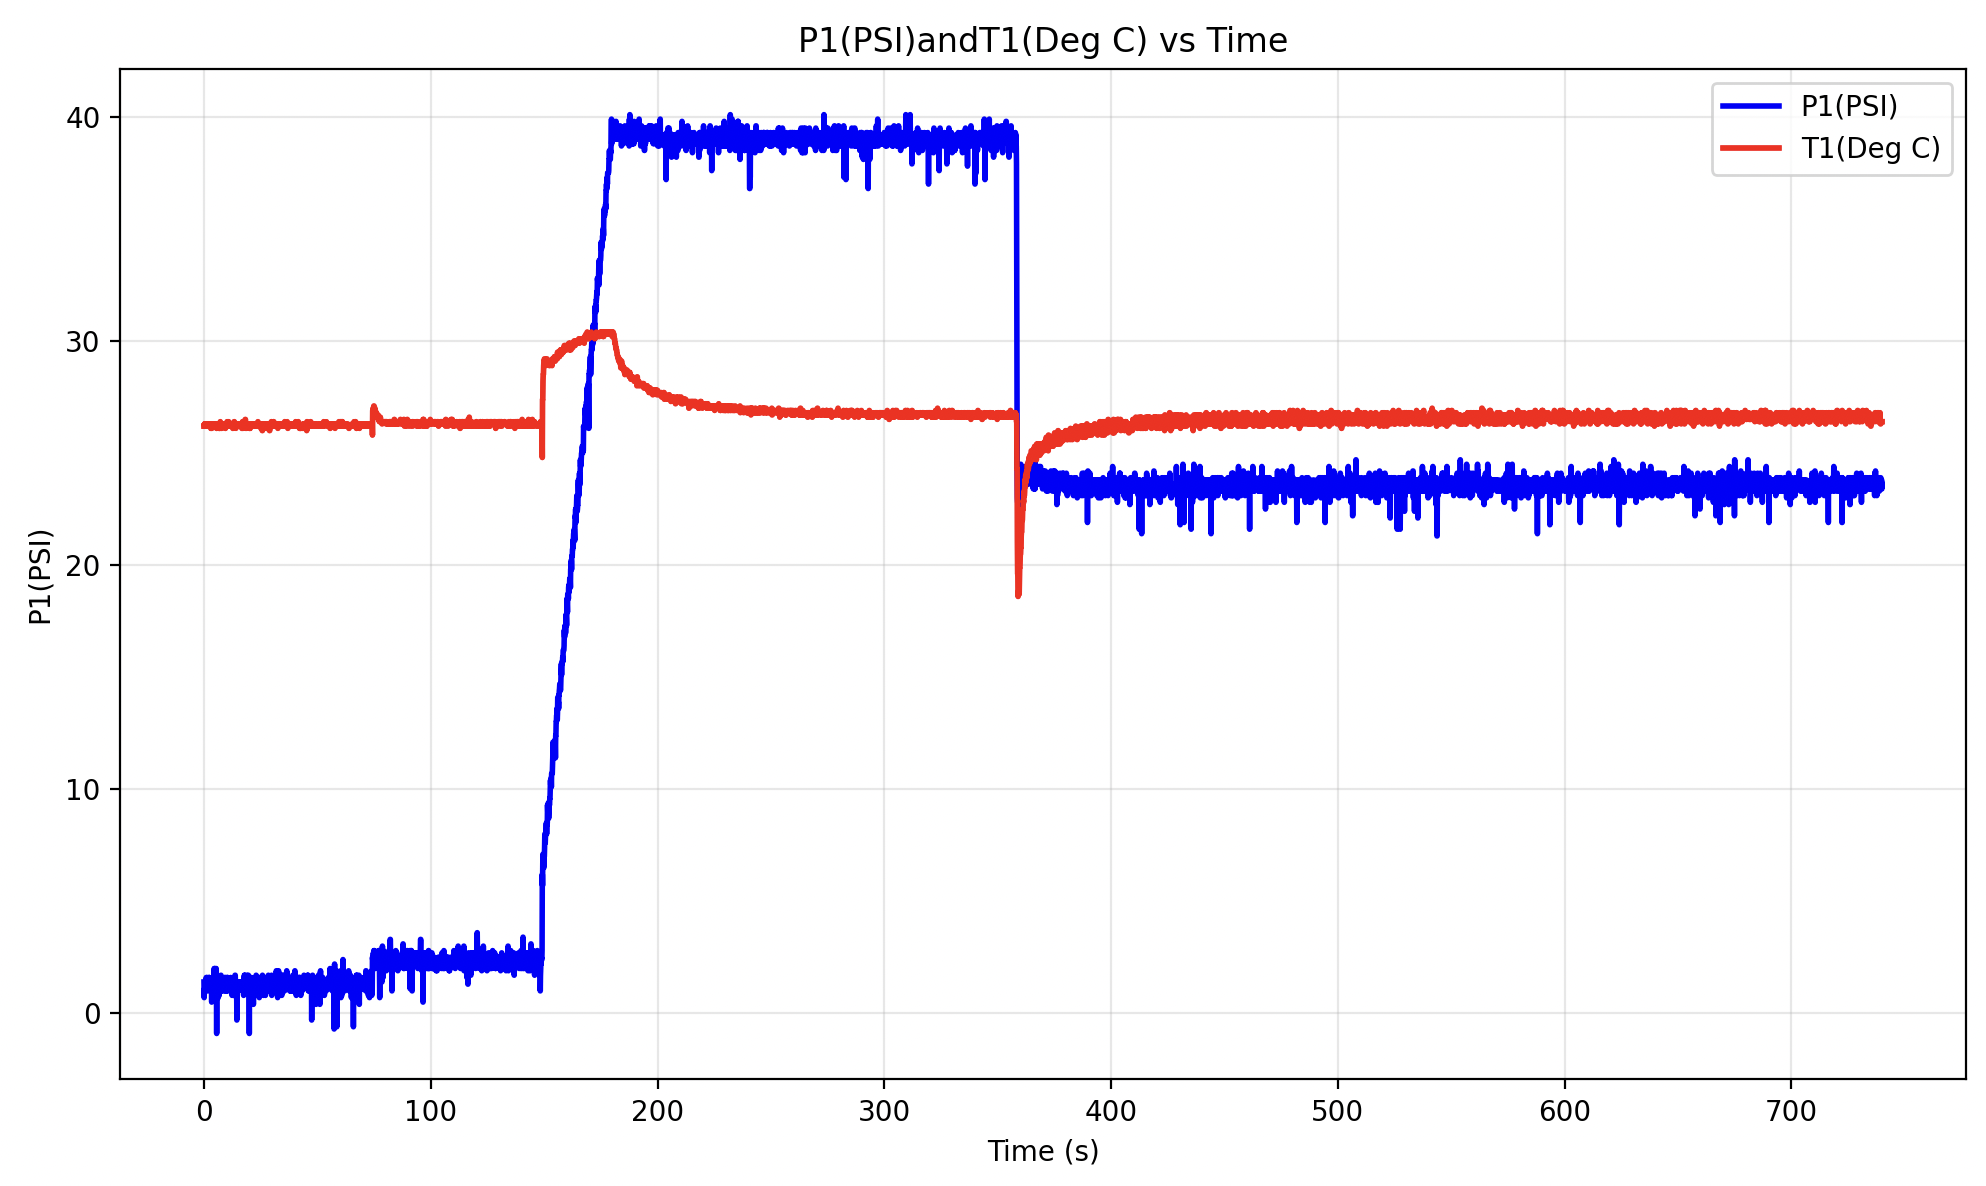
\includegraphics[width=0.8\textwidth]{1a-left_tank.png}
\caption{Pressure (P1) and temperature (T1) measurements for the left tank during Part 1a of the experiment. Around $t = 350$ seconds, the pressure gauge between the tanks is opened, a sharp drop in pressure and temperature visible.}
\label{fig:tank1_data_a}
\end{figure}

\begin{figure}[h!]
\centering
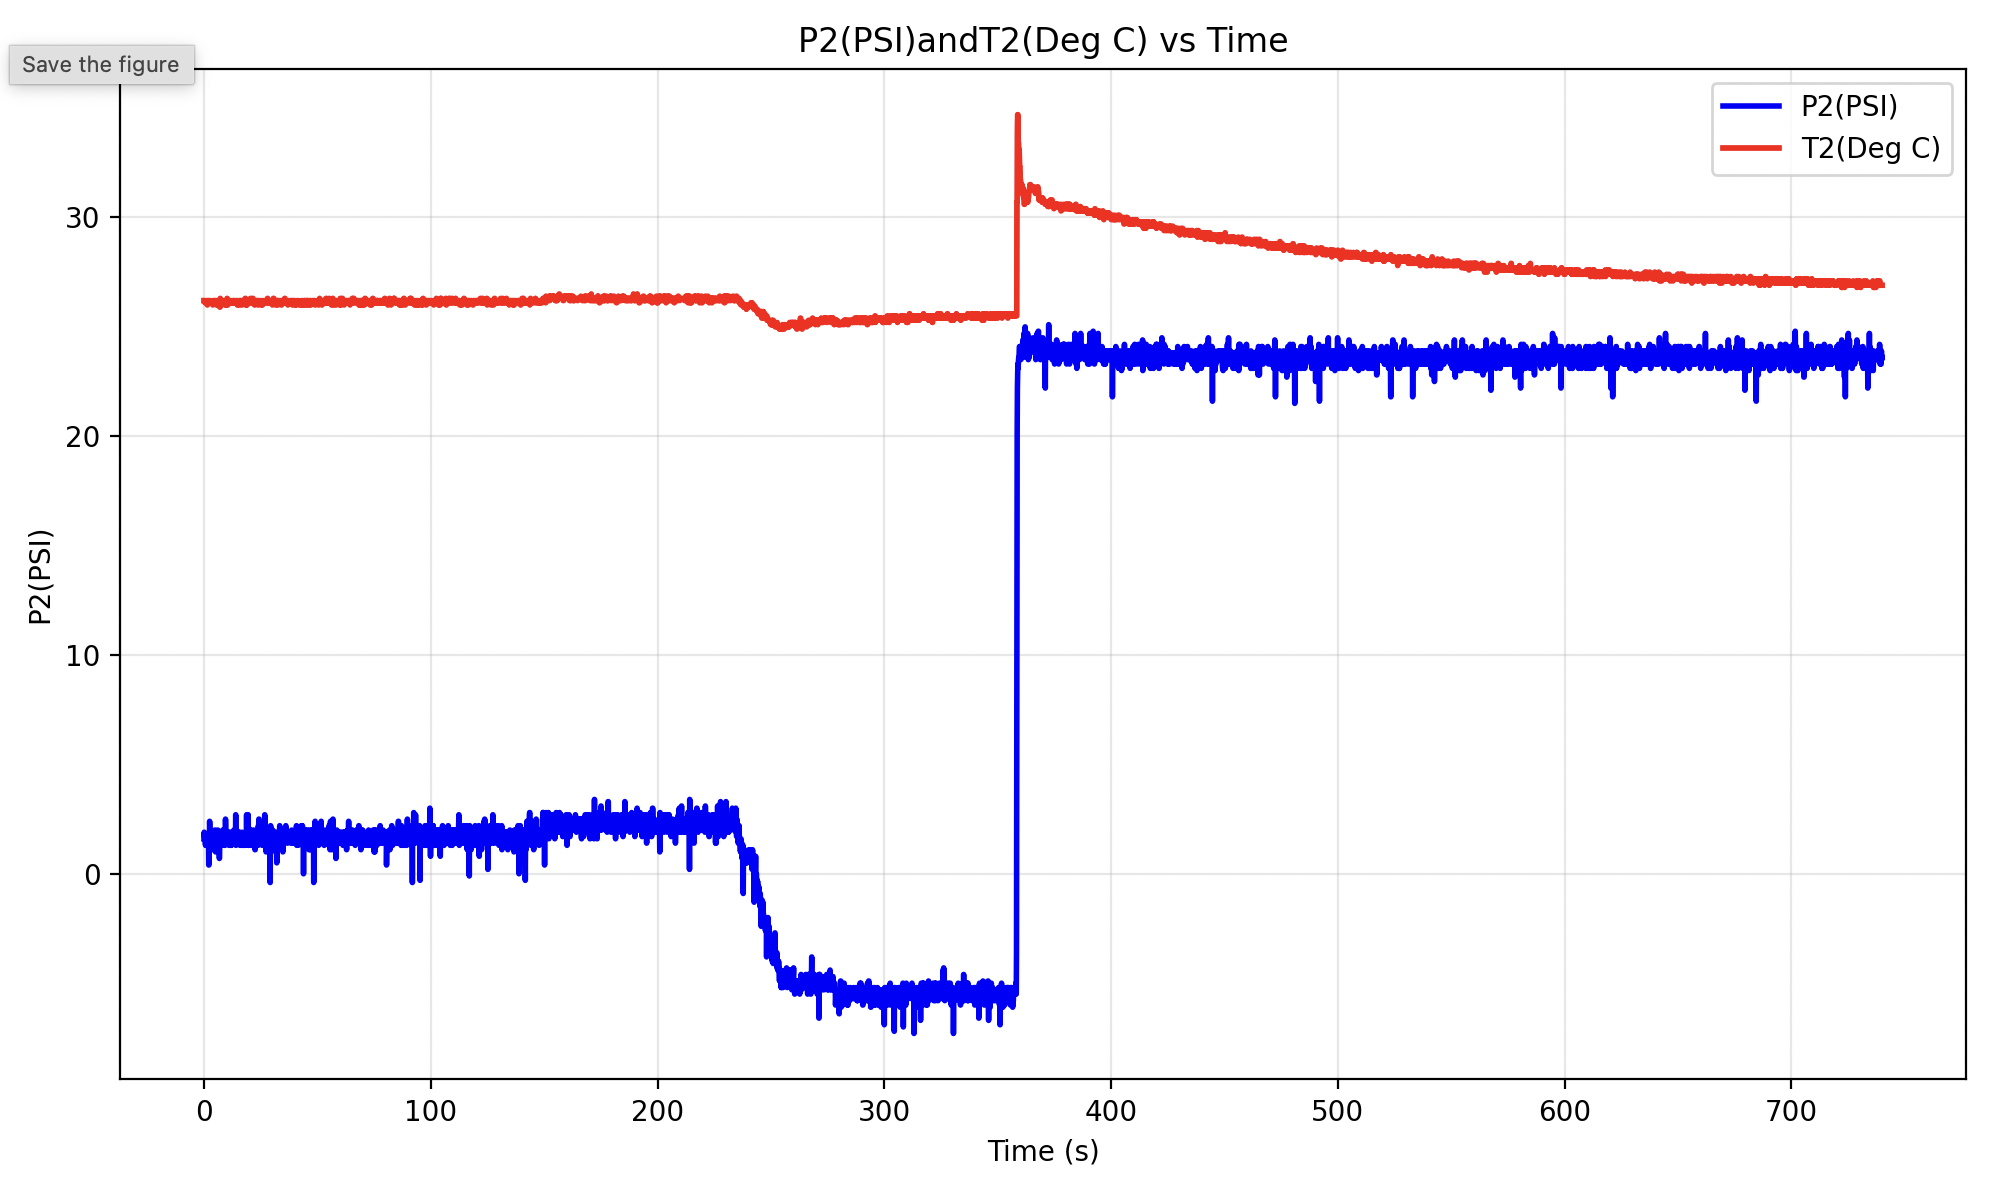
\includegraphics[width=0.8\textwidth]{1a-right_tank.png}
\caption{Pressure (P2) and temperature (T2) measurements for the right tank during Part 1a of the experiment, a sharp rise in pressure and temperature as a result of high-pressure gas from the left tank being released.}
\label{fig:tank2_data_a}
\end{figure}

\newpage
Substituting the measured pressures as shown in Figure~\ref{fig:tank1_data_a} ($P_1 = 39.0~\text{psi}$, $P_f = 23.6~\text{psi}$):
\[ \frac{V_2}{V_1} = \frac{39.0}{23.6} - 1 \approx 1.6525 - 1 = 0.6525 \approx 0.653 \]
Thus, the right tank has about 0.653 times the volume of the left tank (equivalently, $V_1/V_2 \approx 1.533$).

\subsection*{Net Heat Transfer}
In both expansion cases, heat transfer occurs between the tanks and their surroundings as the system moves toward equilibrium. 
In the first case, when the pressures of the two chambers are rapidly equalized, the high-pressure gas in the left tank expands quickly into the right tank, causing a sharp drop in temperature due to the rapid expansion (a process approximating an adiabatic expansion) (see Figure 2). 
Over time, the cold gas in both tanks absorbs heat from the environment until the system returns to room temperature, as shown by the red line in Figure~\ref{fig:tank1_data_a}. This results in a positive net heat transfer from the surroundings to the system.

\begin{figure}[h!]
\centering
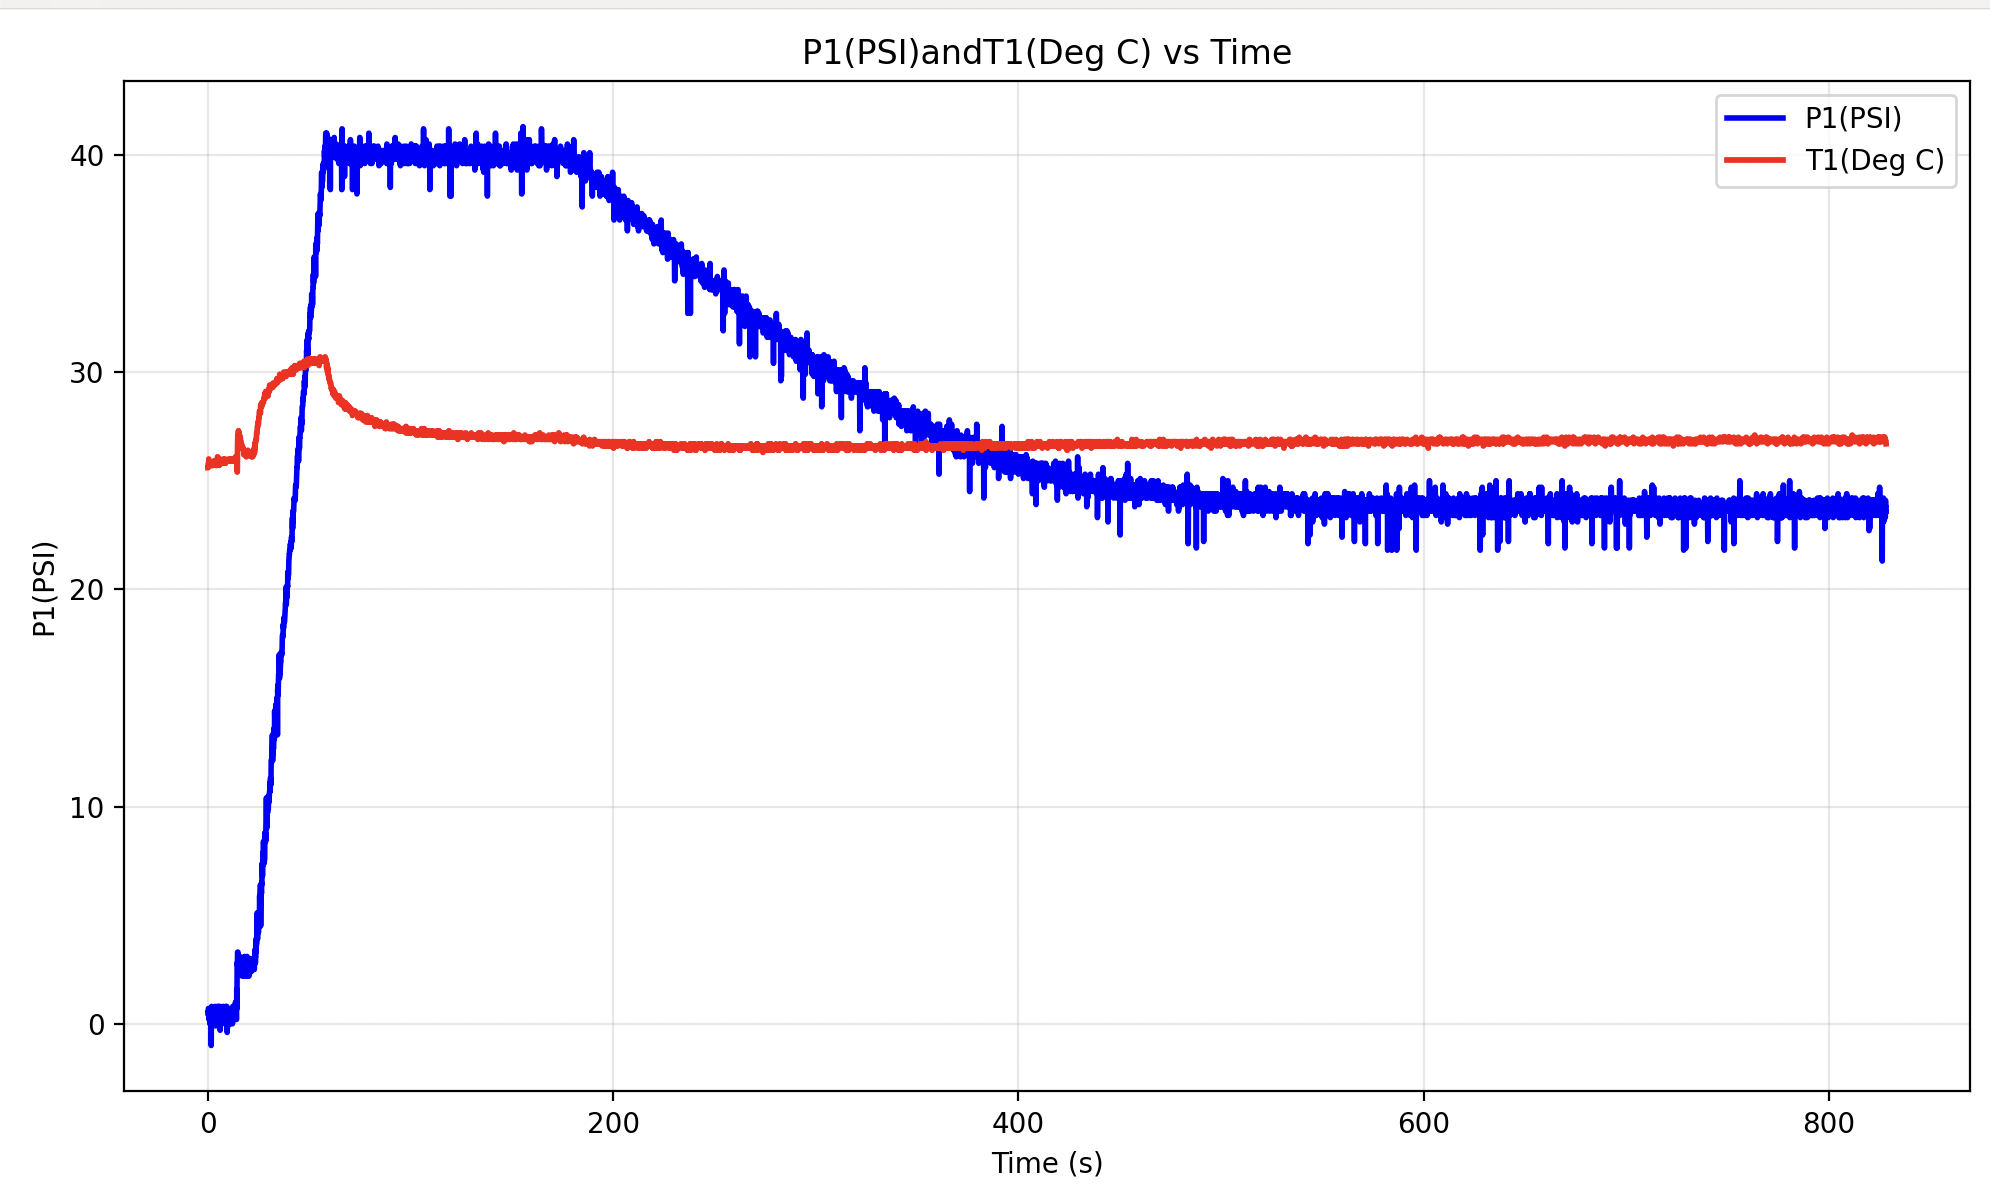
\includegraphics[width=0.8\textwidth]{1b-left_tank.png}
\caption{Pressure (P1) and temperature (T1) measurements for the left tank during Part 1b of the experiment. The small gauge is opened at around $t=200$. As gas is slowly released, the pressure in this tank decayed exponentially.}
\label{fig:tank1_data_b}
\end{figure}

\begin{figure}[h!]
\centering
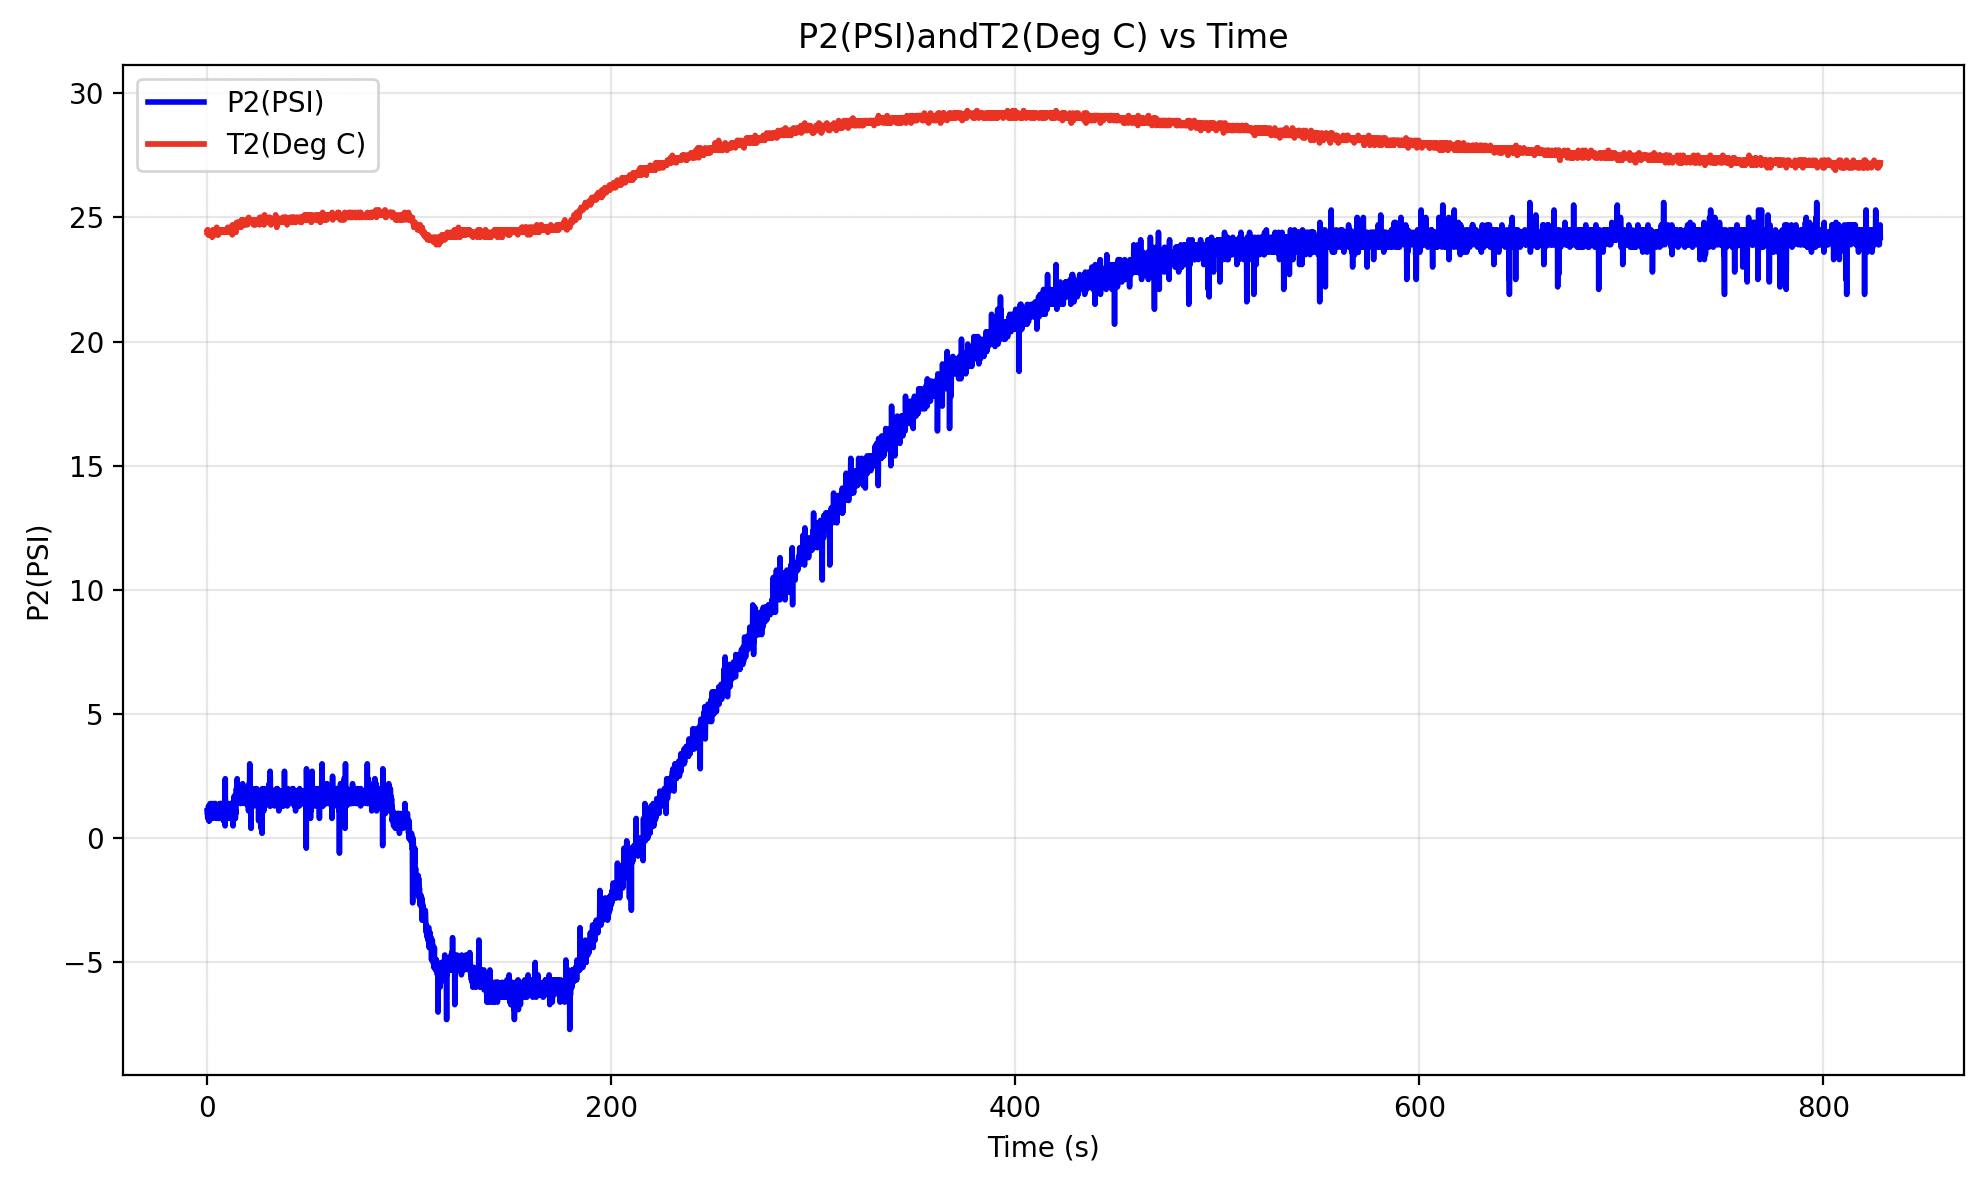
\includegraphics[width=0.8\textwidth]{1b-right_tank.png}
\caption{Pressure (P2) and temperature (T2) measurements for the right tank during Part 1b of the experiment. The small gauge is opened at around $t=200$. As gas is slowly released, the pressure in this tank approached equilibrium pressure.}
\label{fig:tank2_data_b}
\end{figure}

In the second case, the expansion occurs slowly and is essentially isothermal, meaning the temperature remains constant. As the gas in the left tank expands gradually into the right tank, the expanded gas tends to cool, but it continuously absorbs heat from the surroundings to maintain room temperature ~\ref{fig:tank2_data_b}. Simultaneously, the left tank also becomes cooler as it loses pressure and absorbs heat from the environment ~\ref{fig:tank2_data_a}. Therefore, in both cases, the net heat transfer is positive, with heat flowing from the surroundings into the system to bring the gas to thermal equilibrium with the environment.

\subsection*{Path Independence of State Properties}
This experiment demonstrates that state properties are path independent because, although the gas expansion occurs differently in the two cases—rapidly in the first (approaching adiabatic) and slowly in the second (approaching isothermal)—the system reaches the same final equilibrium state in both situations, with equal pressure and temperature in the two tanks. The difference lies only in how heat is exchanged during the process: in the rapid expansion, the gas first cools and then absorbs heat from the surroundings, while in the slow expansion, the gas continuously absorbs heat to maintain a constant temperature. Despite these different paths, the final state of the system is identical, showing that state properties such as pressure, temperature, and internal energy depend only on the initial and final conditions, not on the process by which the system changes.

\subsection*{Calculated Mass and Volume}

The initial mass of the left tank was calculatedthrough integrating the mass flow rate with respect to time. A left-hand Riemann-sum with Python \cite{integrate_script} yielded a total of \SI{0.030496}{\kilogram} of air transferred, as shown in figure ~\ref{fig:massintegration}.
\begin{figure}[h!]
\centering
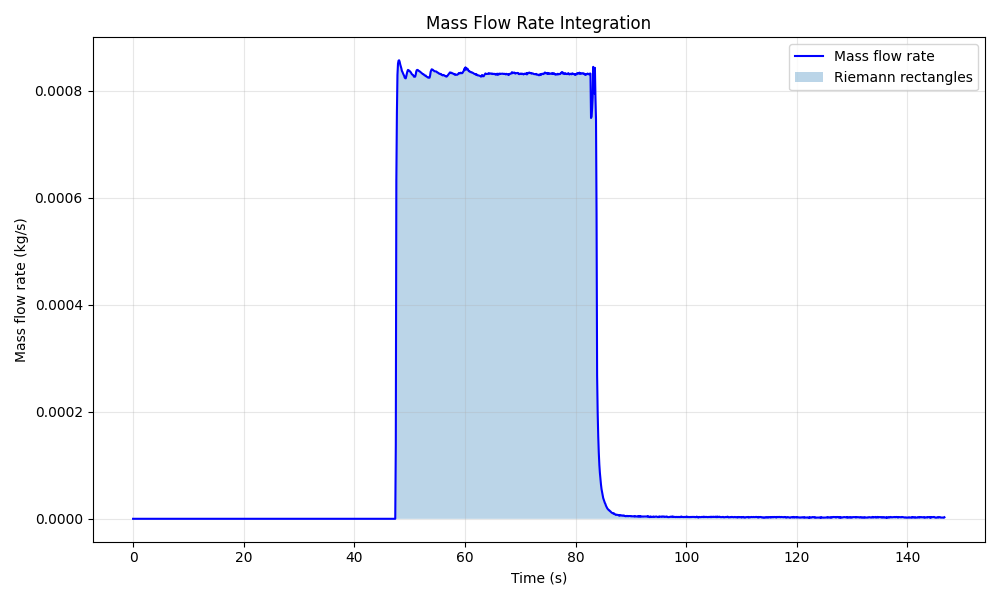
\includegraphics[width=0.8\textwidth]{massintegration.png}
\caption{Total mass of air transferred, calculated using left-hand Riemann sum integration of the mass flow rate data.}
\label{fig:massintegration}
\end{figure}
The measured gauge pressure was \SI{272.34}{\kPa}, which was converted to absolute pressure by adding atmospheric pressure (\SI{101.3}{\kPa}) to give \(P_{abs} = 272.34 + 101.3 = \SI{373.64}{\kPa}\). Substituting this value and the measured conditions (\(P = 373.64~\si{kPa}\), \(T = 300.3~\si{K}\)) into the Ideal Gas Law gave:
\[
V = \frac{mRT}{P} =
\frac{(0.030496)(0.287)(300.3)}{373.64} =
\SI{7.007e-3}{\metre\cubed}.
\]
Thus, the left-tank volume was approximately \SI{7.01}{\litre}.


\subsection*{Error Analysis}
Primary uncertainties arose from (1) pressure-gauge calibration drift, (2) human reading error on the manometer, (3) thermocouple lag, and (4) noise in the flow-rate sensor.  

To estimate uncertainty in the calculated mass, pressure and flow rate were assumed to have respective uncertainties of \(\pm1~\si{psi}\) and \(\pm0.5~\si{g/min}\). 
Propagation through Eq.~(3) gives a combined relative uncertainty of approximately \(3\%\). 
This aligns with the spread in repeated integrations using the Python script. 
Pressure uncertainty contributes most strongly to the overall error in \(Z\).  

The estimated uncertainty in the total mass was \(\pm 3\%\), dominated by flow-meter fluctuations.  
The compressibility factor was found to be \(Z = 0.997 \pm 0.003\), which deviates from unity by less than experimental uncertainty, confirming that air behaved ideally under these conditions.
This small deviation is expected, as air at room temperature and moderate pressure typically exhibits near-ideal behavior and is typically modelled as such.


Because air behaves nearly ideally at moderate pressures and room temperature, deviations from \(Z=1\) fall within the expected range of experimental uncertainty.

\section*{Conclusion}
The Riemann-sum integration of mass-flow-rate data successfully determined the total mass of air transferred between tanks. The derived tank volume (\SI{7.007e-3}{\metre\cubed}) and compressibility factor near unity confirmed the validity of the Ideal Gas Law for air at room temperature and moderate pressure. The Python-based numerical method provided an accurate and reproducible approach for integrating experimental data. Future improvements should focus on reducing sensor lag and improving gauge calibration to minimize uncertainty.

\begin{thebibliography}{9}
\bibitem{che260_manual}
CHE260 Course Notes, \textit{Ideal Gas Law Laboratory Manual}. Toronto: University of Toronto, 2025.

\bibitem{che260_guidelines}
CHE260 Course Handout, \textit{Lab Report Guidelines}. Toronto: University of Toronto, 2025.

\bibitem{engineering_toolbox}
Engineering Toolbox, ``Air Properties and Gas Constant.'' [Online]. Available: \url{https://www.engineeringtoolbox.com}. [Accessed: Oct. 8, 2025].

\bibitem{integrate_script}
K. Peng, B. Zhang, and Y.Y. Zhang, ``Mass flow integration script,'' \textit{integrate.py}. [Online]. Available: \url{https://github.com/YYZ-CR/CHE260-Lab/blob/main/idealgaslab/data/integrate.py}. [Accessed: Oct. 8, 2025].
\end{thebibliography}

\end{document}
